\documentclass[letterpaper,12pt]{article}

\usepackage{tabularx} % extra features for tabular environment
\usepackage{amsmath}  % improve math presentation
\usepackage{amssymb}
\usepackage{multirow}
\usepackage{xcolor}
\usepackage{gensymb}
\usepackage{appendix}
\usepackage{gensymb}
\usepackage{float}
\usepackage{listings}
\usepackage[export]{adjustbox}
\usepackage{graphicx} % takes care of graphic including machinery
\usepackage[margin=1in,letterpaper]{geometry} % decreases margins
\usepackage{cite} % takes care of citations
\usepackage[final]{hyperref} % adds hyper links inside the generated pdf file
\newcommand*{\tran}{^{\mkern-1.5mu\mathsf{T}}}

\hypersetup{
    colorlinks=false,       % false: boxed links; true: colored links
    linkcolor=blue,        % color of internal links
    citecolor=blue,        % color of links to bibliography
    filecolor=magenta,     % color of file links
    urlcolor=blue         
}
%++++++++++++++++++++++++++++++++++++++++++++++++++++++++++++++++++++++++++++++++



%++++++++++++++++++++++++++++++++++++++++++++++++++++++++++++++++++++++++++++++++
% Start modifying the labwork number, your team number and the name and METU id
% of your group members.
\newcommand{\reporttitle}{Problem Set 2}
\newcommand{\reportauthor}{ Volkan Aydıngül (Id: 0075359 )\\
                            }
                            % If any teammate does not help to write this report,
                            % you may not write his/her name here.
%++++++++++++++++++++++++++++++++++++++++++++++++++++++++++++++++++++++++++++++++



%++++++++++++++++++++++++++++++++++++++++++++++++++++++++++++++++++++++++++++++++
% DO NOT MODIFY THIS SECTION
\begin{document}
\begin{titlepage}
\newcommand{\HRule}{\rule{\linewidth}{0.5mm}}
\begin{center} % Center remainder of the page
%	LOGO SECTION

\includegraphics[width = 8cm]{figures/koc_logo.png}

%	HEADING SECTIONS
\textsc{\Large PHYS 514 - Computational Physics}\\[1.5cm] 
%	TITLE SECTION
\HRule \\[0.6cm]
{ \huge \bfseries \reporttitle}\\ % Title of your document
\HRule \\[1.5cm]
\end{center}
\vspace{2cm}
%	AUTHOR SECTION
\begin{flushleft} \large
\textit{Author:}\\
\reportauthor% Your name
\end{flushleft}
\vspace{2cm}
\makeatletter
Date: \@date 
\vfill % Fill the rest of the page with whitespace
\makeatother
\end{titlepage}
%++++++++++++++++++++++++++++++++++++++++++++++++++++++++++++++++++++++++++++++++




\tableofcontents
\newpage





%\begin{figure}[H] 
%   \centering \includegraphics[width=\columnwidth]{figures/figure.png}           
%                \caption{Caption}                
%                   \label{fig:label}
%   \end{figure}

\section{Problem V}
\subsection{Solution of Linear System vs. Minimization Problem}
\paragraph{} We are given the following function:
\begin{equation}
   \label{eqn:minProb}
   f(\mathbf{x}) =\frac{1}{2} \mathbf{x} \tran A \mathbf{x} - \mathbf{b} \mathbf{x}
\end{equation}
Moreover, we are asked to investigate relation between the minimization of above equation and solving below linear system.
\begin{equation}
   \label{eqn:linSys}
   A\mathbf{x} = \mathbf{b}
\end{equation}
First, let's consider the minimization problem. So as to find the $\mathbf{x}$ value that minimizes the $f(\mathbf{x})$, we need to look up its derivative.
\begin{equation*}
   \frac{\partial f}{\partial \mathbf{x}} = A\mathbf{x} - \mathbf{b}
\end{equation*}
Given that Eqn. \ref{eqn:symDer} is true when the $A$ is symmetric.
\begin{equation}
   \label{eqn:symDer}
   \frac{\partial  \mathbf{x} \tran A \mathbf{x} }{\partial \mathbf{x}} = 2A\mathbf{x}
\end{equation}
\paragraph{}At this point, one need to consider the following relation to be able to infer minimum value of $\mathbf{x}$.
\begin{equation}
   \label{eqn:min0}
   \frac{\partial f}{\partial \mathbf{x}} = \mathbf{0} = A\mathbf{x} - \mathbf{b}
\end{equation}
Finally, the solution of the Eqn. \ref{eqn:min0} is equivalent of the solution of the Eqn. \ref{eqn:linSys}. Therefore, we can conclude that minimization of the Eqn. \ref{eqn:minProb} is same as with the solution of Eqn. \ref{eqn:linSys} if the $A$ is symmetric and positive definite.

\subsection{Finding the Optimal Learning Rate in Gradient Descent Algorithm}
\paragraph{}For a given function $f(\mathbf{x})$ to be minimized, the gradient descent algorithm can be written in a following way:
\begin{equation*}
   \mathbf{x}_{n+1} = \mathbf{x}_n - \tau \nabla f(\mathbf{x}_n)
\end{equation*}
From Eqn. \ref{eqn:min0}, $\nabla f(\mathbf{x}_n)$ is known for our case:
\begin{equation*}
   \nabla f(\mathbf{x}_n) = A\mathbf{x}_n - \mathbf{b}
\end{equation*}
\paragraph{} However, there emerges a question that what is the optimal value of learning rate ($\tau$)? To provide an answer for this question, we need to investigate the rate of change of next estimation of the function ($f(\mathbf{x})$) with respect to learning rate ($\tau$), which is formulated below:

\begin{equation}
   \label{eqn:tauDep}
\frac{\partial f(\mathbf{x}_{n+1})}{\partial \tau} = \frac{\partial f(\mathbf{x}_{n+1})}{\partial \mathbf{x}_{n+1}} \frac{\mathbf{x}_{n+1}}{\partial \tau}
\end{equation}

To obtain a stable algorithm, Eqn. \ref{eqn:tauDep} should be zero, which means that the estimation of function should not be dependent on learning rate. One can easily compute that:
\begin{equation*}
   \frac{\partial f(\mathbf{x}_{n+1})}{\partial \mathbf{x}_{n+1}} =  \nabla f(\mathbf{x}_{n+1})
\end{equation*} 
\begin{equation*}
   \frac{\mathbf{x}_{n+1}}{\partial \tau} = - \nabla f(\mathbf{x}_n)
\end{equation*}

To sum up, we obtain:
\begin{equation*}
   \nabla f(\mathbf{x}_{n+1}) \tran \left( - \nabla f(\mathbf{x}_n) \right) = 0
\end{equation*}

Let's dive in this equation for much more detail.
\begin{equation*}
   \left( A\mathbf{x}_{n+1} - \mathbf{b} \right) \tran \left( A\mathbf{x}_{n} - \mathbf{b} \right) = 0
\end{equation*}
Let's say $\mathbf{\alpha}_n = A\mathbf{x}_{n} - \mathbf{b}$, and continue with this notation for simplicity, without attributing a meaning.
\begin{equation*}
\left( A \left( \mathbf{x}_n - \tau \mathbf{\alpha}_n \right) - \mathbf{b} \right) \tran \mathbf{\alpha}_n = 0
\end{equation*}

\begin{equation*}
   \left( A\mathbf{x}_n - A \tau \mathbf{\alpha}_n - \mathbf{b} \right) \tran \mathbf{\alpha}_n = 0
\end{equation*}
\begin{equation*}
   \left( A \mathbf{x}_n - \mathbf{b} \right) \tran \mathbf{\alpha}_n - \left( A \tau \mathbf{\alpha}_n \right)\tran \mathbf{\alpha}_n = 0
\end{equation*}

\begin{equation*}
   \left( A \mathbf{x}_n - \mathbf{b} \right) \tran \mathbf{\alpha}_n = \tau \left( A \mathbf{\alpha}_n \right)\tran \mathbf{\alpha}_n 
\end{equation*}

\begin{equation*}
   \mathbf{\alpha}_n \tran \mathbf{\alpha}_n = \tau \left( A \mathbf{\alpha}_n \right)\tran \mathbf{\alpha}_n 
\end{equation*}
\begin{equation*}
   \mathbf{\alpha}_n \tran \mathbf{\alpha}_n = \tau \mathbf{\alpha}_n \tran \left( A \mathbf{\alpha}_n \right)
\end{equation*}
\begin{equation*}
   \boxed{\tau = \frac{ \mathbf{\alpha}_n \tran \mathbf{\alpha}_n}{\mathbf{\alpha}_n \tran  A \mathbf{\alpha}_n }}
\end{equation*}

\subsection{Gauss-Seidel Method}
   \paragraph{}As we have done in \textit{Jacobi Method}, again, we decompose the $A$ matrix into parts. In \textit{Gauss-Seidel Method}, the $A$ matrix can be expressed as following:
   \begin{equation*}
      A = L_* + U
   \end{equation*}
   where $L_*$ is the lower triangular part of the $A$ matrix, and $U$ is the strictly upper triangular part of the $A$ matrix.
   \paragraph{}Suppose that the $\mathbf{x}^*$ is the solution of the linear system of $A\mathbf{x} = \mathbf{b}$. Then, one can write the following relation:
   \begin{equation*}
      L_* \mathbf{x}^* = \mathbf{b} - U \mathbf{x}^*
   \end{equation*}
   Finally, the iterative scheme can be obtained as following:
   \begin{equation*}
      \mathbf{x}^{(k+1)}=  L_*^{-1} \left(\mathbf{b} - U \mathbf{x}^{(k)}\right) 
   \end{equation*}

   \subsection{Time Comparison of Different Methods and Matrix Types}
   
\begin{figure}[H] 
   \centering 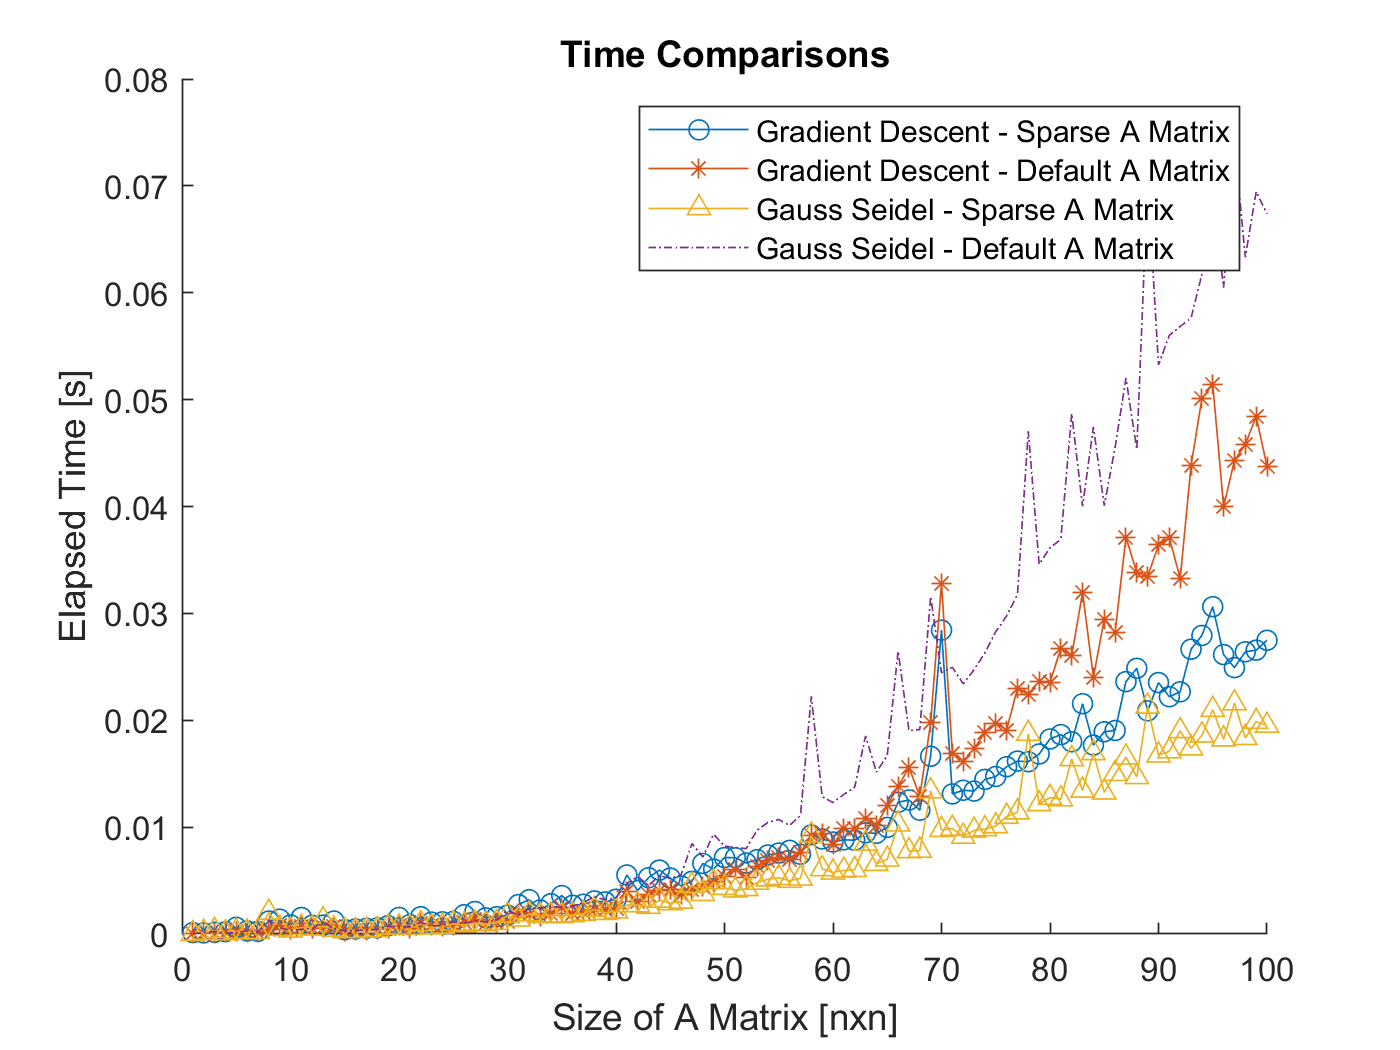
\includegraphics[width=\columnwidth]{figures/linsystime.png}           
                \caption{Time Comparison}                
                   \label{fig:linsystime}
   \end{figure}
   As can be seen from Figure \ref{fig:linsystime}, when we use the \textit{sparse matrix} constructor of the \textit{MATLAB}, we can obtain better performance. If want to analyze Figure \ref{fig:linsystime} in terms of solution methods, we can easily conclude that \textit{Gauss-Seidel Method} shows superiority over \textit{Gradient-Descent Method}. However, at the same time, the poorest performance is provided by the \textit{Gauss-Seidel Method}, which is processed with \textit{default matrix} constructor.
\begin{figure}[H] 
   \centering 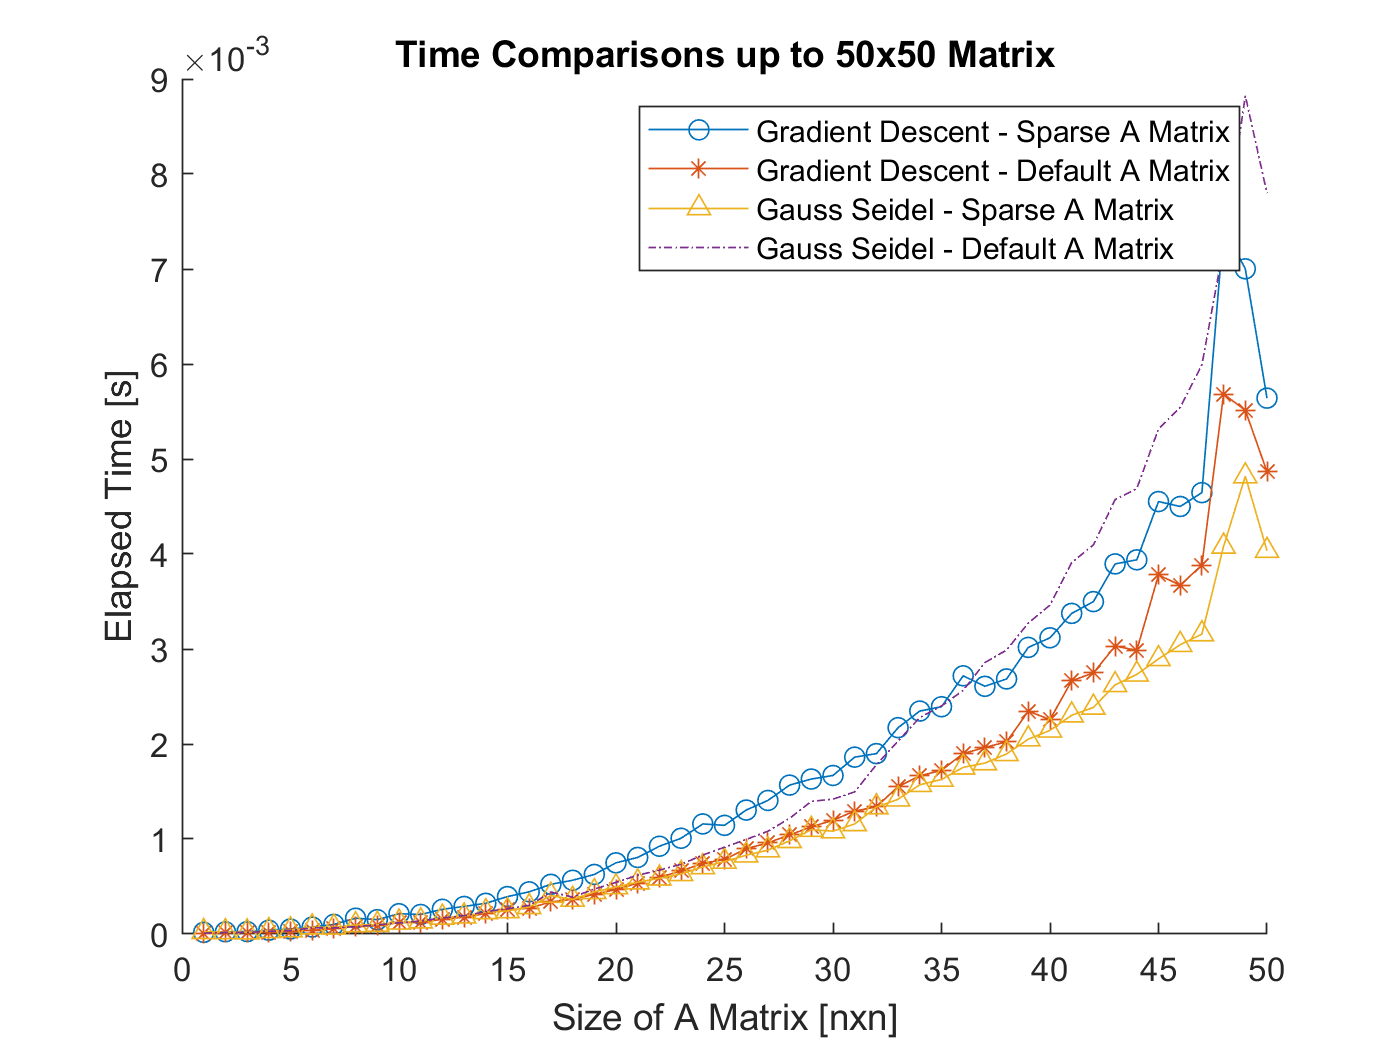
\includegraphics[width=\columnwidth]{figures/linsystime50.png}           
                  \caption{Time Comparison}                
                     \label{fig:linsystime50}
   \end{figure}
   \paragraph{}Moreover, from Figure \ref{fig:linsystime50}, we can observe when we simulate the time comparisons up to $50\times50$ matrix, the similar trend with Figure \ref{fig:linsystime} can not be displayed. For example, in this case, the superiority of the \textit{sparse matrix} is not valid for the \textit{Gradient-Descent Method}.
   
   
\section{Problem VI}
\subsection{Time Comparisons of Function Evaluations}
\paragraph{} In the question/code template, we are given the main algorithm in a element-by-element manner. We can display two evidence for that:
\begin{itemize}
   \item In the inline function definition, broadcast operator (.) is not used.
   \item Initial value of x determined as a scalar value.
\end{itemize}
\paragraph{} These factors should definitely reduce the performance of the algorithm. To avoid from this draw-back, we can process all algorithm in a element-wise manner. Also, for example, as an ending criteria of the algorithm, we can use the difference of the norm of the solution vectors rather than using the difference between two scalar guesses. Below in Figure \ref{fig:lamberttime}, the time comparisons of different algorithms can be observed.
\begin{figure}[H] 
   \centering 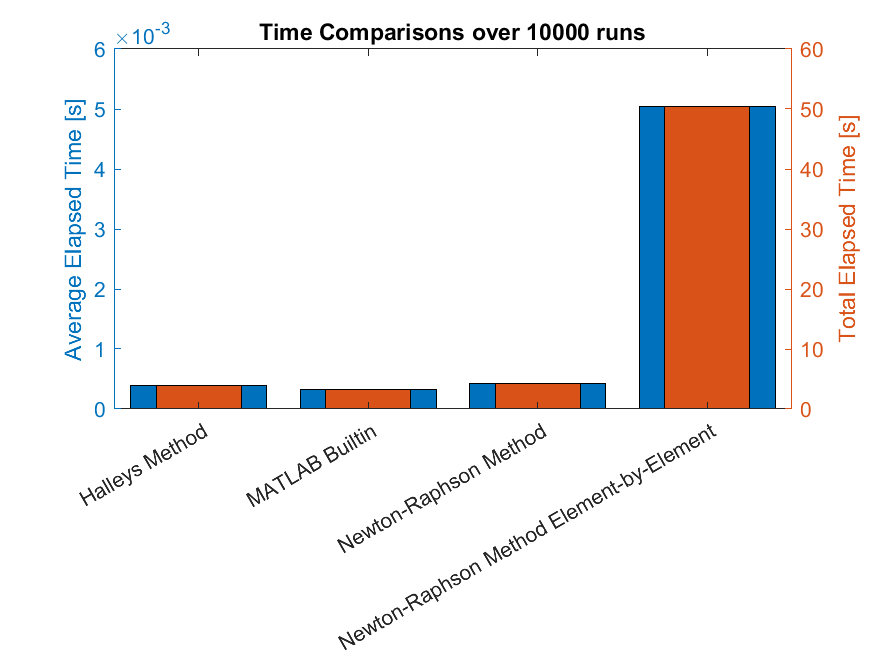
\includegraphics[width=0.5\columnwidth]{figures/lamberttime.png}           
                  \caption{Time Comparison of Lambert W Function Evluations}                
                     \label{fig:lamberttime}
   \end{figure}
As can be seen from Figure \ref{fig:lamberttime}, the element-by-element operation results in dramatic performance reduction.
\begin{figure}[H] 
   \centering 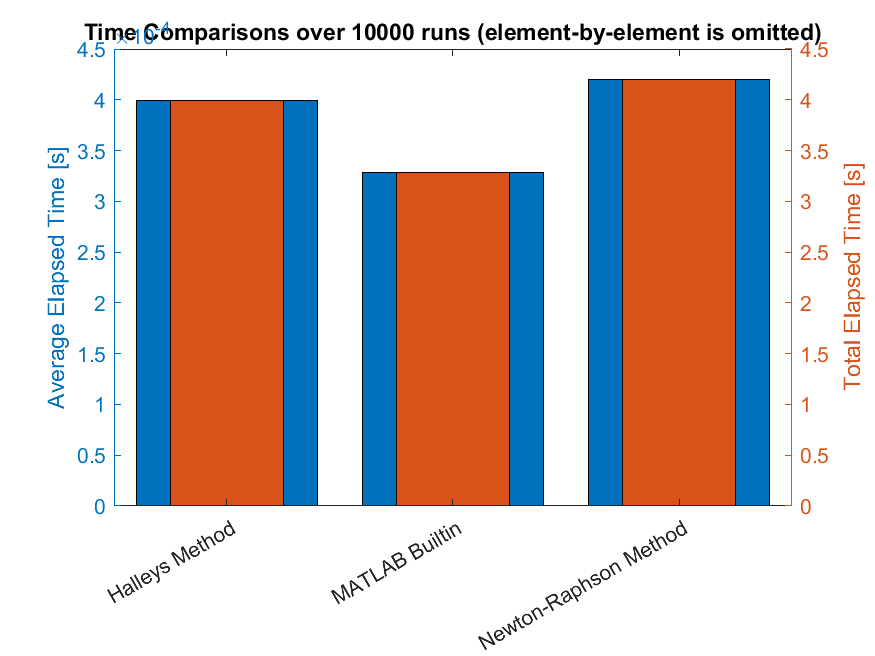
\includegraphics[width=0.7\columnwidth]{figures/lamberttimedetailed.png}           
                  \caption{Time Comparison of Lambert W Function Evluations in Detail}                
                     \label{fig:lamberttimedetailed}
   \end{figure}
   In Figure \ref{fig:lamberttimedetailed}, the time comparisons of algorithms (element-by-element operation is omitted) can be displayed. Here, we can observe the similarity between the algorithms we implemented and the built-in MATLAB function. In Figure \ref{fig:lamberttime} and Figure \ref{fig:lamberttimedetailed}, the left y-axis represents the average elapsed time, while the right y-axis represents the total elapsed time over $N$ number of runs.
   \subsection{Function Evaluations}
   From Figure \ref{fig:lambertfunceval}, we can evaluate the \textit{Newton-Raphson Method} and \textit{Halley's Method} are able to approximate \textit{Lambert W} function with a great accuracy. It can be observed from the Figure \ref{fig:lambertfunceval} that nearly all the time, the difference between \textit{Newton-Raphson Method} and \textit{Halley's Method} and MATLAB is zero.
   
\begin{figure}[H] 
   \centering 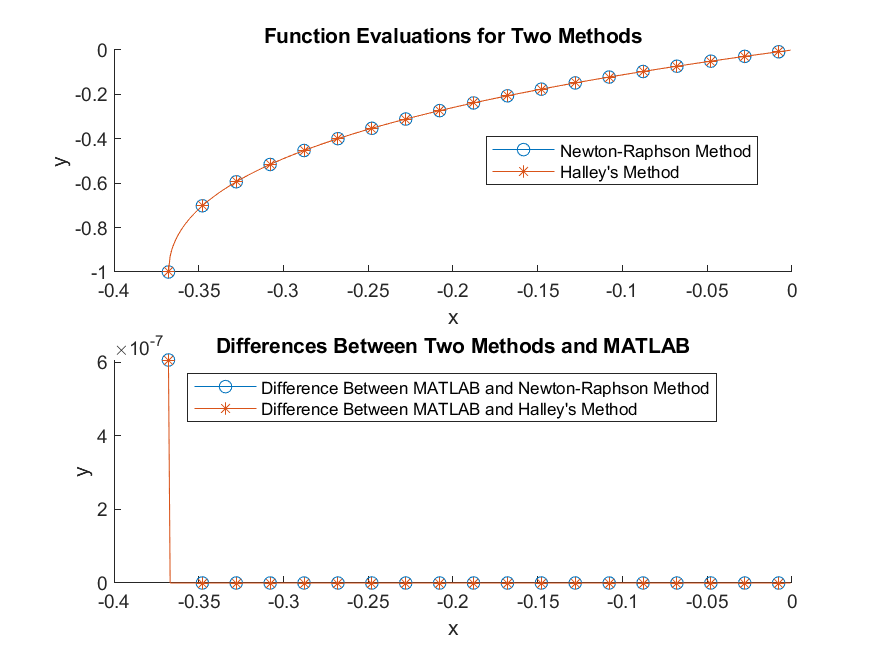
\includegraphics[width=\columnwidth]{figures/lambertfunceval.png}           
                  \caption{Function Evaluations and Differences w.r.t. MATLAB}                
                     \label{fig:lambertfunceval}
   \end{figure}
\pagebreak
\section{Problem  VII}
\subsection{Hotelling's Deflation}
\paragraph{} We are given an $A$ matrix to find its eigenvalues and eigenvectors. When we apply the \textit{Power Iteration} method, we can find the largest eigenvalue (in absolute value) and the corresponding eigenvector of the $A$ matrix. To be able to find the other eigenvalues and eigenvectors, one can apply the \textit{Hotelling's Deflation} method. First, let's appyl eigendecomposition to the $A$ matrix, then $A$ matrix can be written as following:
\begin{equation*}
   A = Q \Lambda Q^{-1}
\end{equation*}
Now, suppose that A is a symmetric matrix, then following relation holds:
\begin{equation}
   \label{eqn:inveqtrans}
   Q^{-1} = Q \tran
\end{equation}

\begin{equation*}
   A = Q \Lambda Q \tran
\end{equation*}

where $\Lambda$ is the diagonal matrix whose elements are the eigenvalues of the $A$ matrix, and $Q$ is the orthogonal matrix whose columns are the eigenvectors of $A$ matrix.Then, the above relation can be written for $N \times N$ symmetric matrix in this way:
\begin{equation}
   \label{eqn:symmatrix}
   A = \lambda_1 \mathbf{v_1} \mathbf{v_1}\tran + \lambda_2 \mathbf{v_2} \mathbf{v_2}\tran \dots \lambda_N \mathbf{v_N} \mathbf{v_N}\tran  
\end{equation}
where $\lambda$ is the eigenvalue of $A$ matrix and $\mathbf{v}$ is the corresponding eigenvector. Eigenvalues are oriented such that the relation of $\left(\left\lvert \lambda_1\right\rvert > \left\lvert \lambda_2\right\rvert > \dots \left\lvert \lambda_N\right\rvert\right)$ holds.

\paragraph{} Let's construct a \textbf{new} matrix in following way:
\begin{equation}
   \label{eqn:hotelling}
   A^{(1)} = A - \lambda_1 \mathbf{v_1}\mathbf{v_1}\tran
\end{equation}
where $\lambda_1$ is the largest eigenvalue which is obtained from power iteration, and $\mathbf{v_1}$ is the corresponding eigenvector. Then, if we plug the Eqn. \ref{eqn:symmatrix} into Eqn. \ref{eqn:hotelling}, we obtain the following relation:
\begin{equation*}
   A^{(1)} = \lambda_2 \mathbf{v_2} \mathbf{v_2}\tran + \lambda_3 \mathbf{v_3} \mathbf{v_3}\tran \dots \lambda_N \mathbf{v_N} \mathbf{v_N}\tran  
\end{equation*}
where where $\lambda_2$ is the largest eigenvalue of $A^{(1)}$ and, apparently, the second largest eigenvalue of $A$ which are obtained from power iteration. Finally, we can conclude that when we apply the operation in Eqn. \ref{eqn:hotelling}, the new matrix we obtained has the largest eigenvalue such that it is the second largest eigenvalue of the matrix to which we applied operation. As a side note, if the $A$ matrix is not a symmetrix matrix, then we could not use the relation in the Eqn. \ref{eqn:inveqtrans}, and we were not able to construct the whole algorithm.

\subsection{Time Comparisons}
\begin{figure}[H] 
   \centering 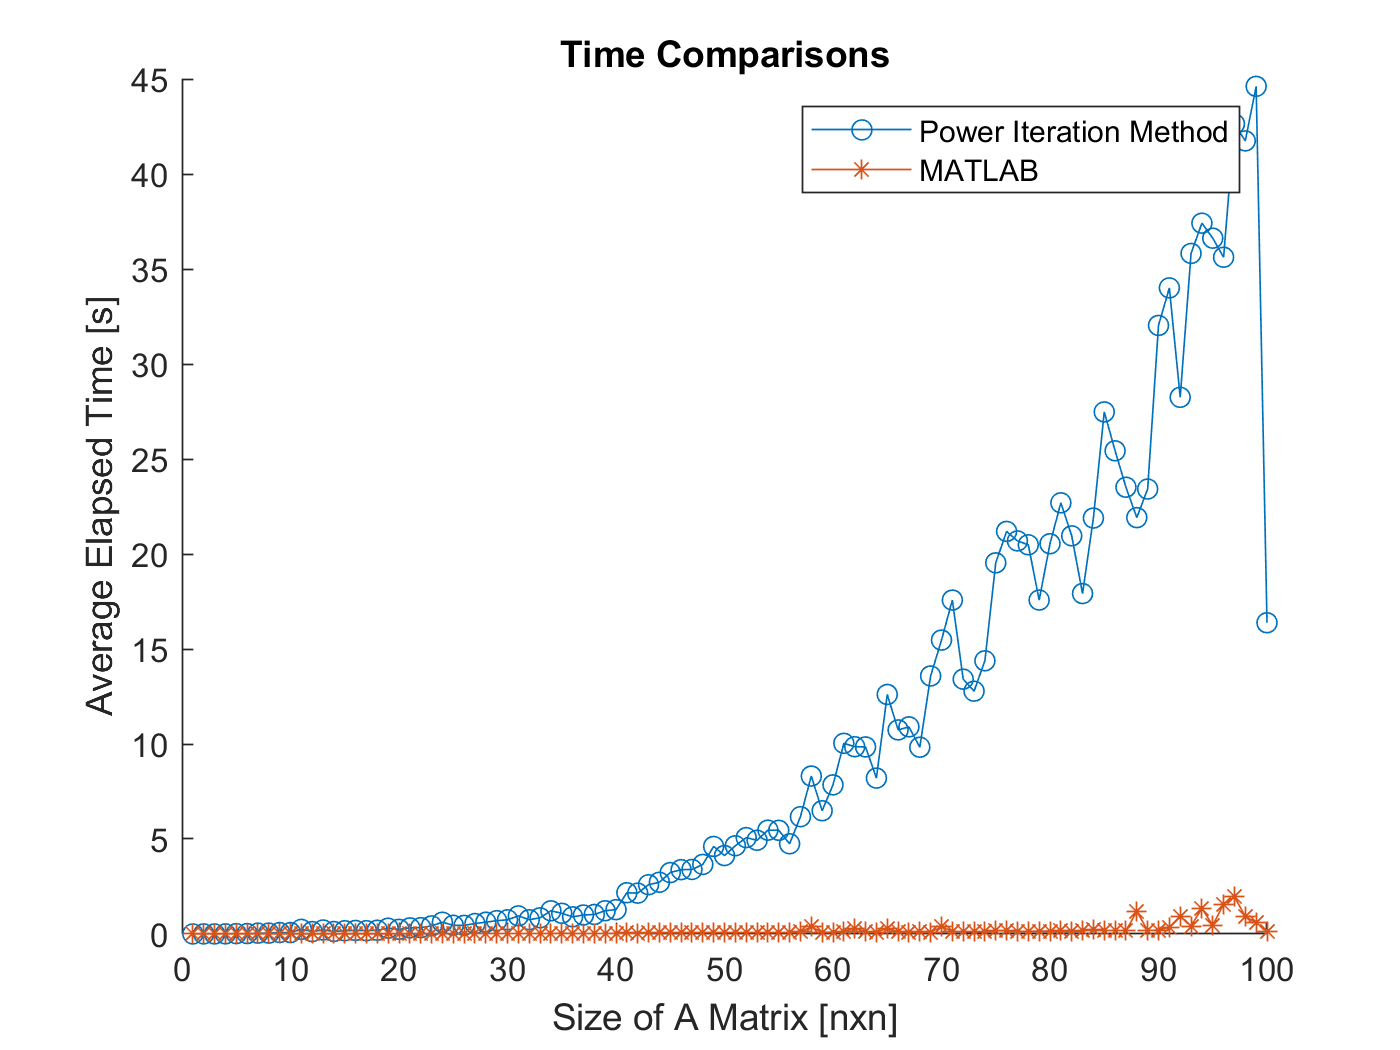
\includegraphics[width=\columnwidth]{figures/poweriterationtime.png}           
                  \caption{Time Comparison Power Iteration Method and Built-in MATLAB \textit{eig()} Function}                
                     \label{fig:poweriterationtime}
   \end{figure}

\paragraph{} As can be seen from the Figure \ref{fig:poweriterationtime}, the pure power iteration algorithm performs very poorly compared to the built-in MATLAB \textit{eig()} function. Generally, the reason for the low performance is the time requirement for the convergence. When we set a low value for accuracy or algorithm termination criteria, the performance is tended to increase, however, in this case, the accuracy is not desirable. For example, below in Figure \ref{fig:poweriterationtimelowtol}, the improvements on the algorithm can be observed, when the accuracy is decreased. 

\begin{figure}[H] 
   \centering 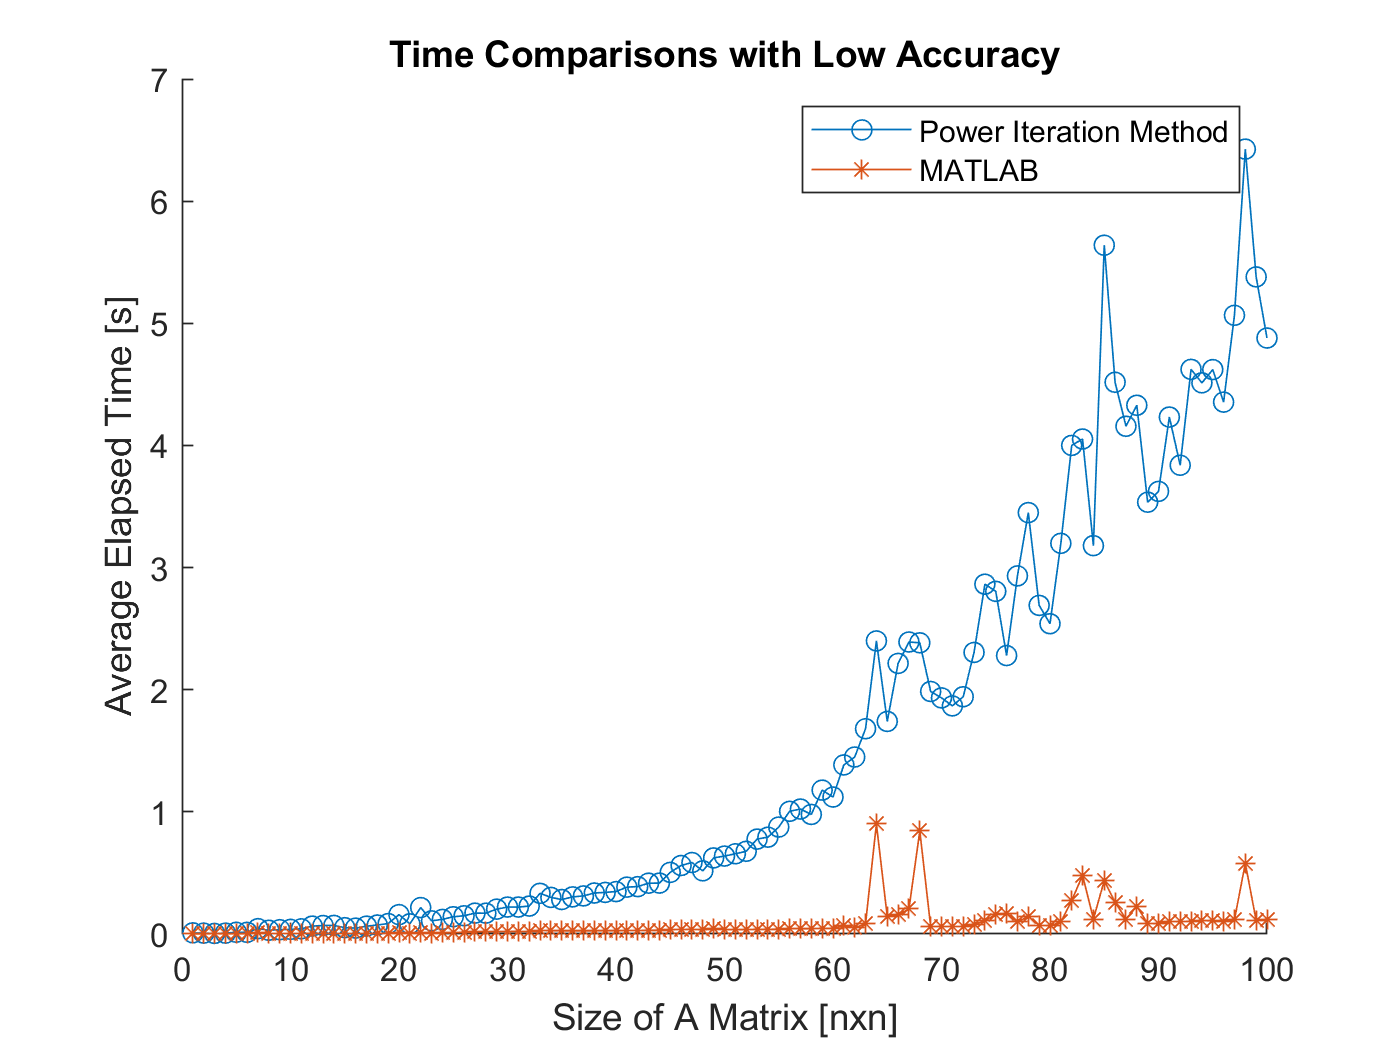
\includegraphics[width=\columnwidth]{figures/poweriterationtimelowtol.png}           
                  \caption{Time Comparison Power Iteration Method and Built-in MATLAB \textit{eig()} Function with Low Accuracy}                
                     \label{fig:poweriterationtimelowtol}
   \end{figure}

   \subsection{Accuracies Compared to MATLAB Built-in}
   \paragraph{}Now, we will examine the accuracy of the eigenvalues and eigenvectors we found. To be able to do this, we will analyze the plots whose x-axis and y-axis are the power iteration solution, and MATLAB solution, respectively. As a side note, all following figures are plotted for a $100 \times 100$ random symmetric matrix. In Figure \ref{fig:eigenvalue}, the accuracies of the eigenvalues estimated by \textit{Power Iteration} method can be observed. At Figure \ref{fig:eigenvalue} and Figure \ref{fig:eigenvector}, the condition to terminate the iteration is to have a proximity of $10^{-7}$ between successive iterations.
\begin{figure}[H] 
   \centering 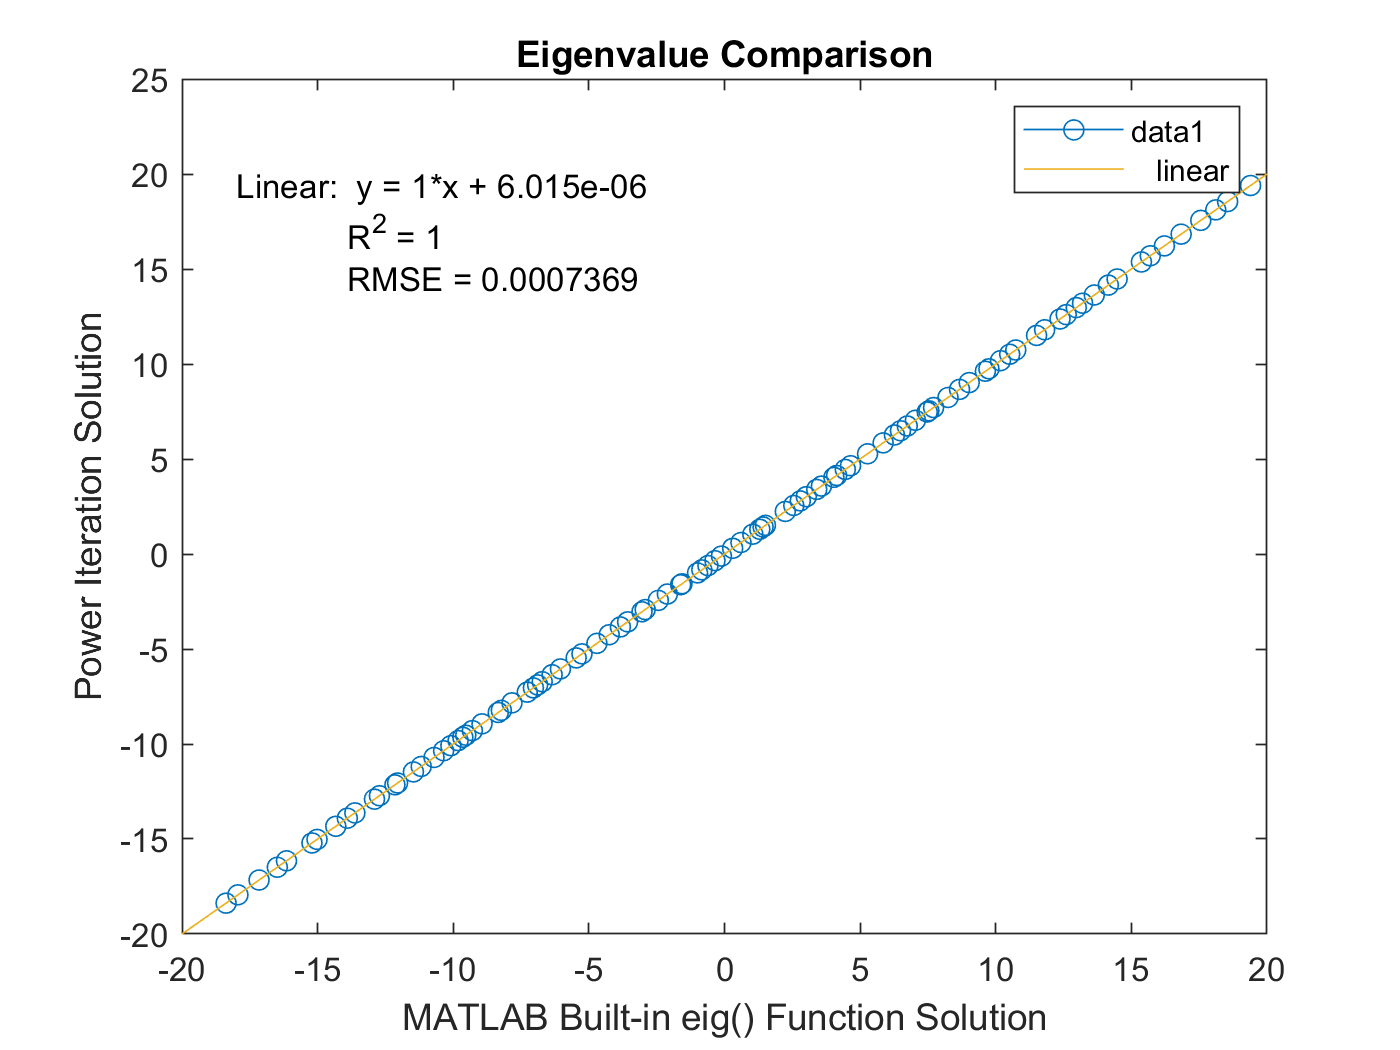
\includegraphics[width=0.7\columnwidth]{figures/eigenvalue.png}           
                  \caption{Accuracy of Eigenvalue Estimation Compared to MATLAB - Termination Condition=$10^{-7}$}                
                     \label{fig:eigenvalue}
   \end{figure}  
   In Figure \ref{fig:eigenvector}, the accuracies of the eigenvectors estimated by \textit{Power Iteration} method can be observed. Again, in this Figure \ref{fig:eigenvector}, the x-axis represents MATLAB estimation, while y-axis represents Power Iteration estimates.
\begin{figure}[H] 
   \centering 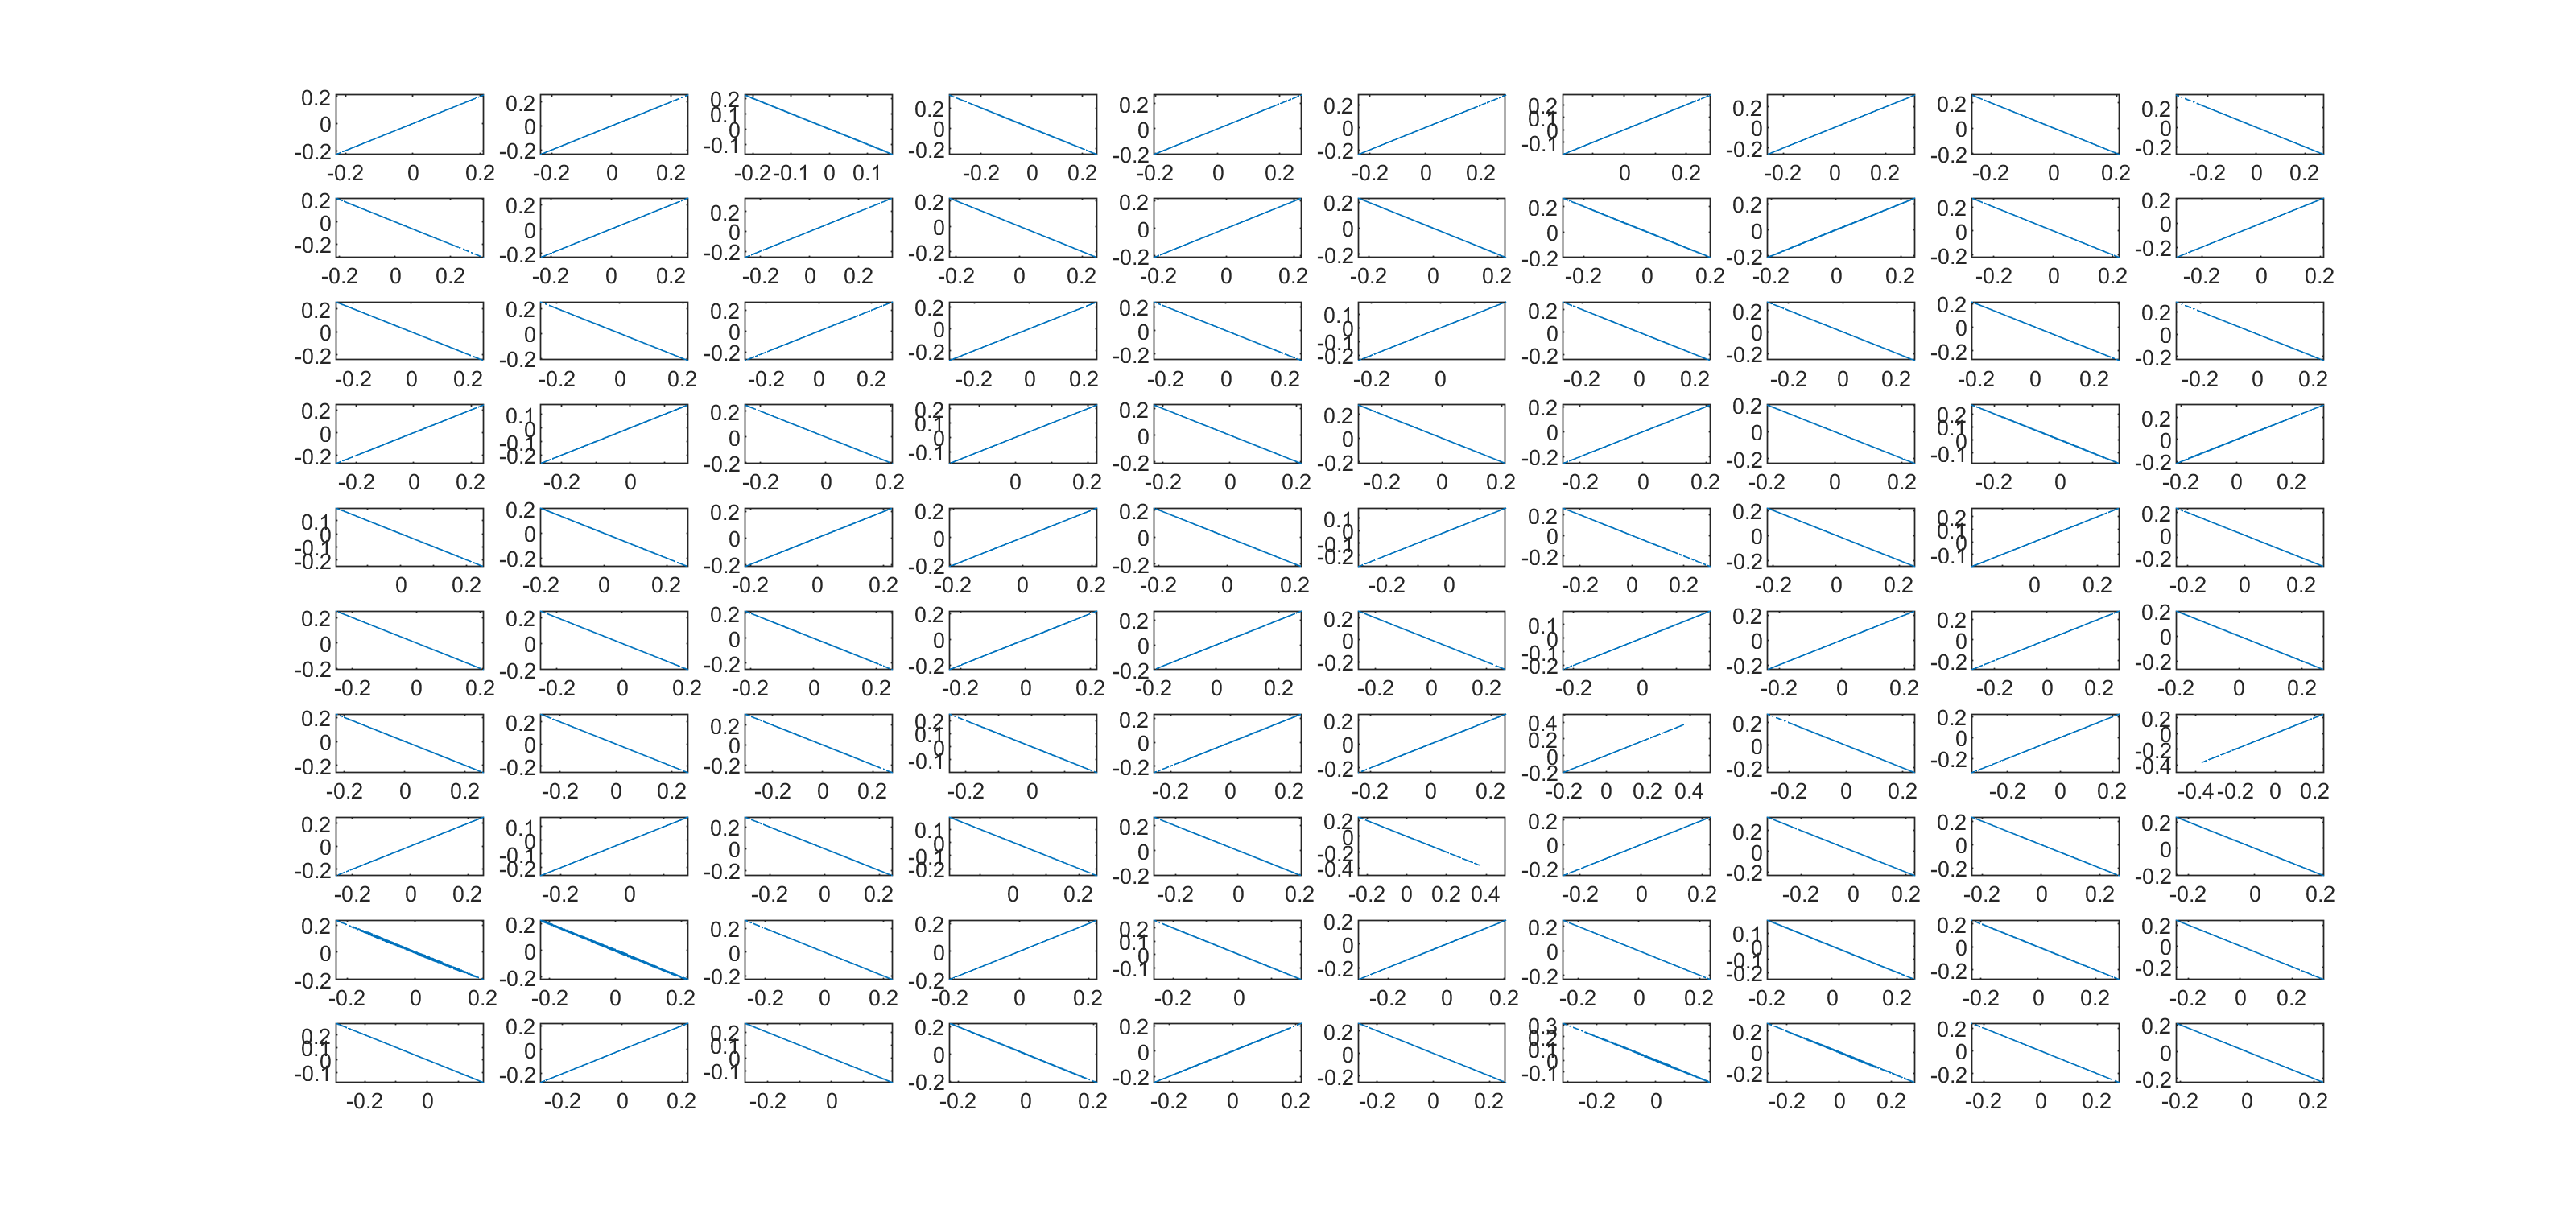
\includegraphics[width=\columnwidth]{figures/eigenvector.png}           
                  \caption{Accuracy of Eigenvector Estimation Compared to MATLAB - Termination Condition=$10^{-7}$}                
                     \label{fig:eigenvector}
   \end{figure}
   \paragraph{} Now we willduplicate the process for a termination condition of $10^{-5}$. Having these condition, Figure \ref{fig:eigenvaluelowacc} and Figure \ref{fig:eigenvectorlowacc} can be displayed. All axis representations and matrix conditions are the same.
   \begin{figure}[H] 
      \centering 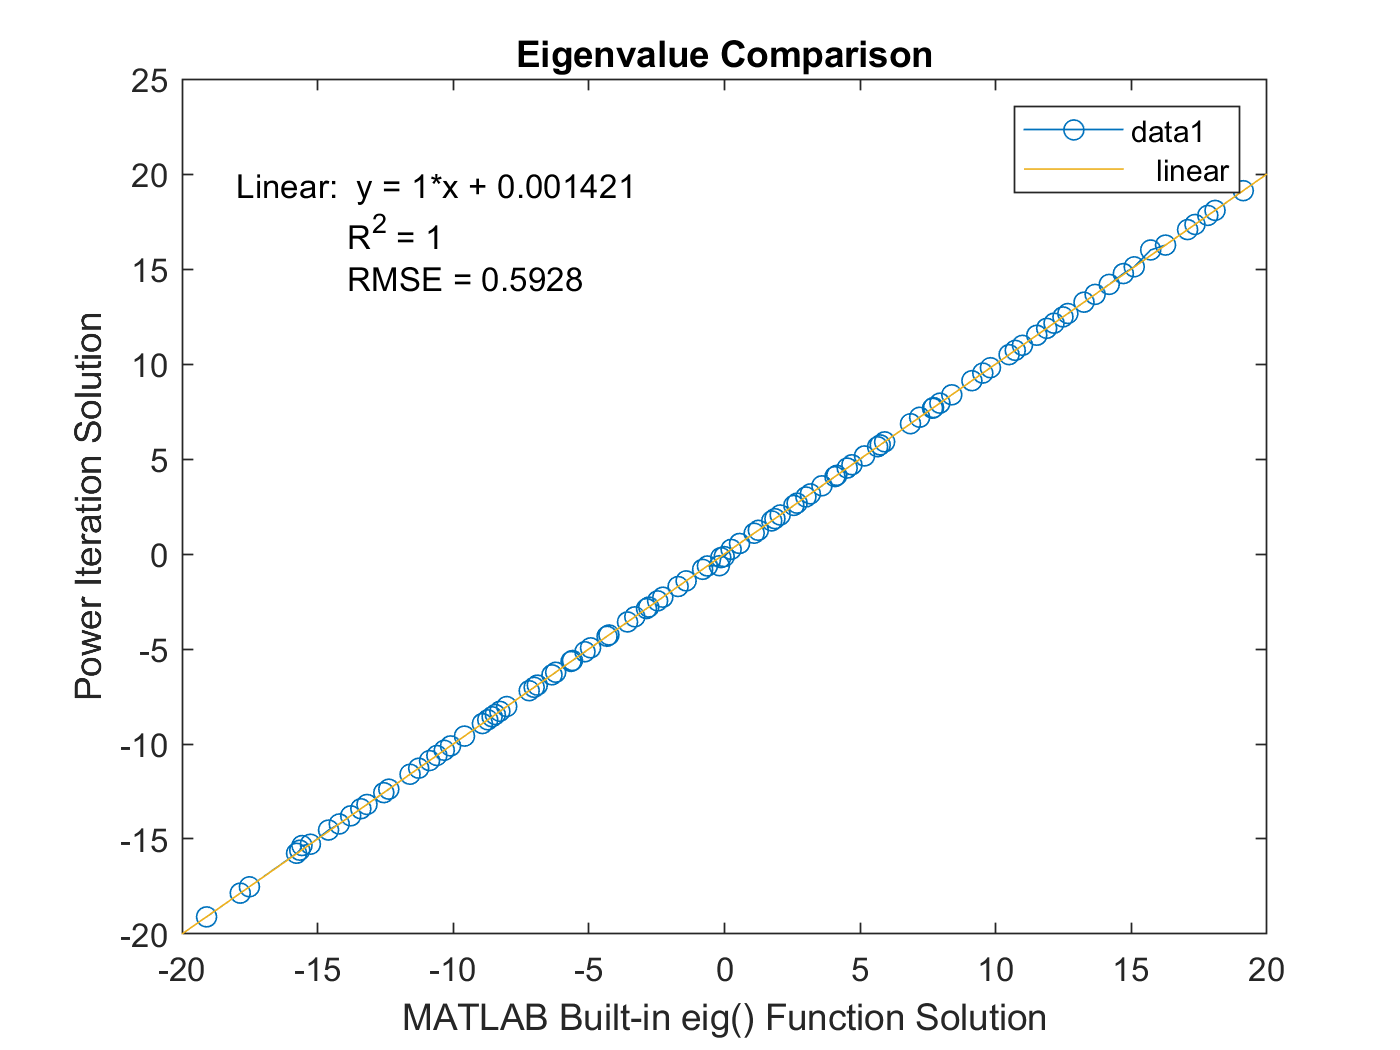
\includegraphics[width=0.7\columnwidth]{figures/eigenvaluelowacc.png}           
                     \caption{Accuracy of Eigenvalue Estimation Compared to MATLAB - Termination Condition=$10^{-5}$}                
                        \label{fig:eigenvaluelowacc}
      \end{figure}  

   \begin{figure}[H] 
      \centering 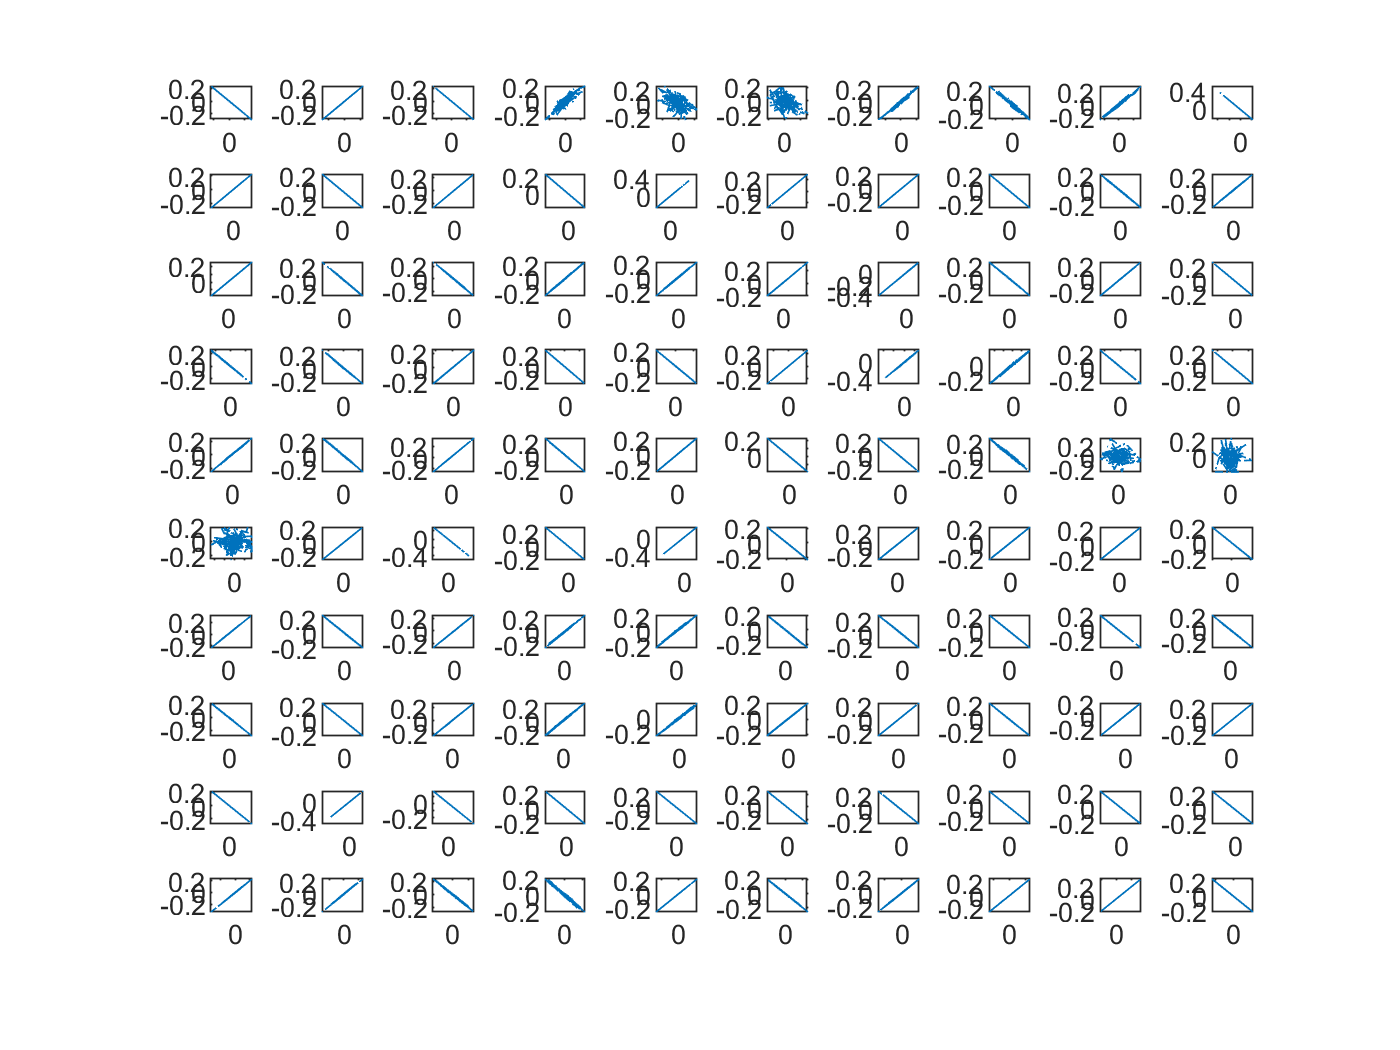
\includegraphics[width=0.7\columnwidth]{figures/eigenvectorlowacc.png}           
                     \caption{Accuracy of Eigenvector Estimation Compared to MATLAB - Termination Condition=$10^{-5}$}                
                        \label{fig:eigenvectorlowacc}
      \end{figure}
      \paragraph{}From Figure \ref{fig:eigenvaluelowacc} and Figure \ref{fig:eigenvectorlowacc}, we can see that while the eigenvalue results are tended to preserve its accuracy, the eigenvectors start to decompose its accuracy. The intricate subplots in the Figure \ref{fig:eigenvectorlowacc} shows this loss of accuracy.
      \paragraph{} By further decreasing termination condition (increasin numerically), we can obtain following Figure \ref{fig:eigenvaluelowlowacc} and Figure \ref{fig:eigenvectorlowlowacc}. Again, all the properties of the figures and matrix are same.
      \begin{figure}[H] 
         \centering 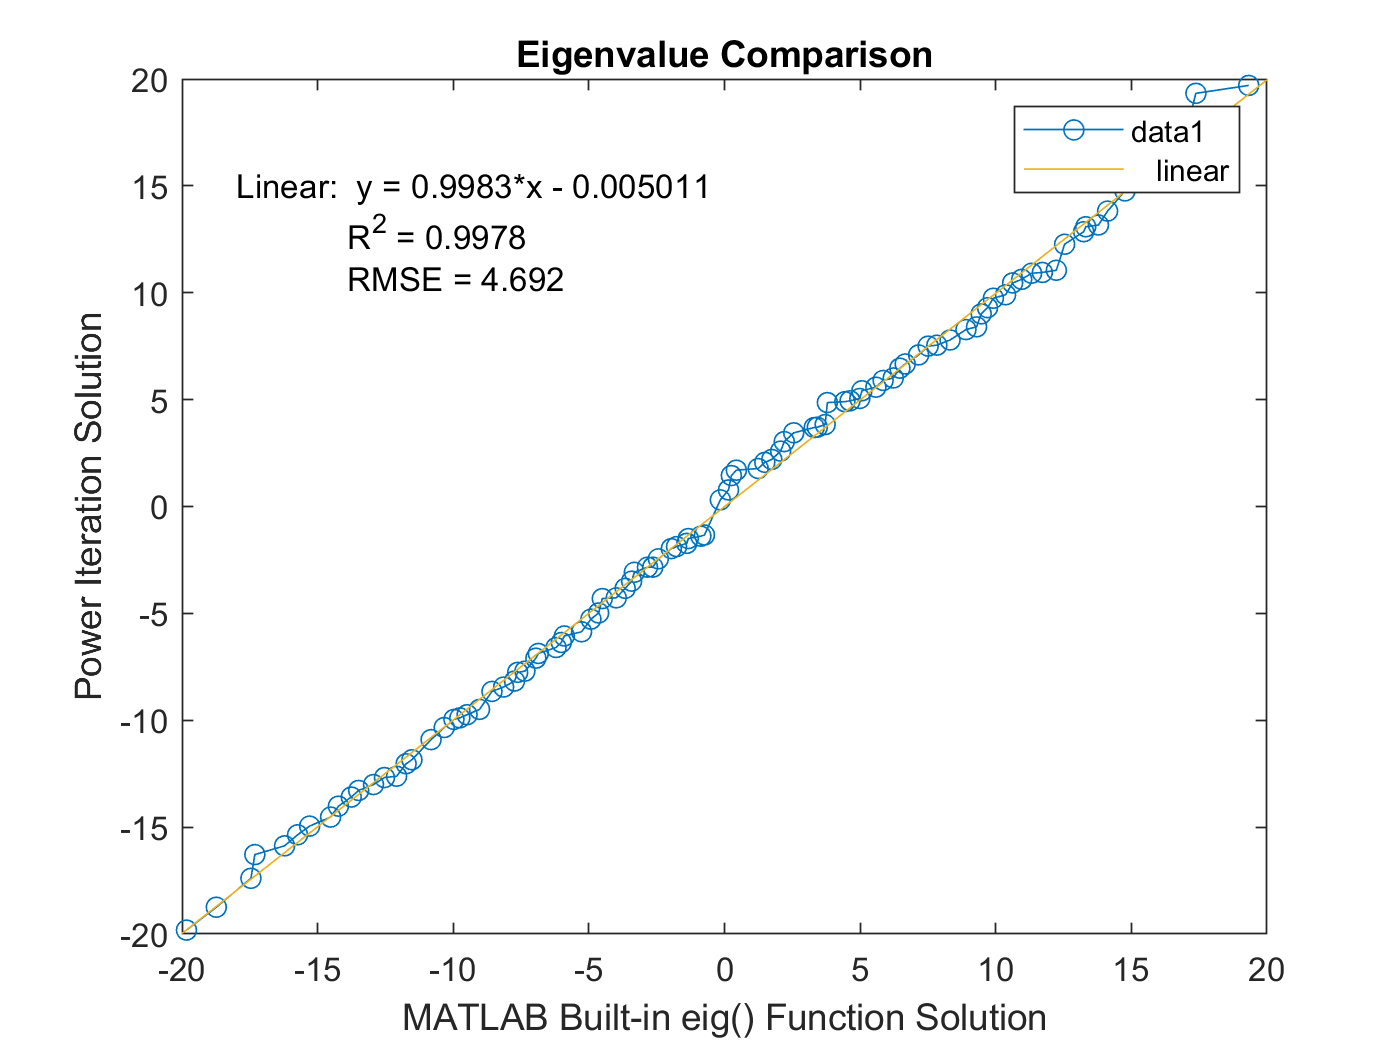
\includegraphics[width=0.7\columnwidth]{figures/eigenvaluelowlowacc.png}           
                        \caption{Accuracy of Eigenvalue Estimation Compared to MATLAB - Termination Condition=$10^{-3}$}                
                           \label{fig:eigenvaluelowlowacc}
         \end{figure}  
   
      \begin{figure}[H] 
         \centering 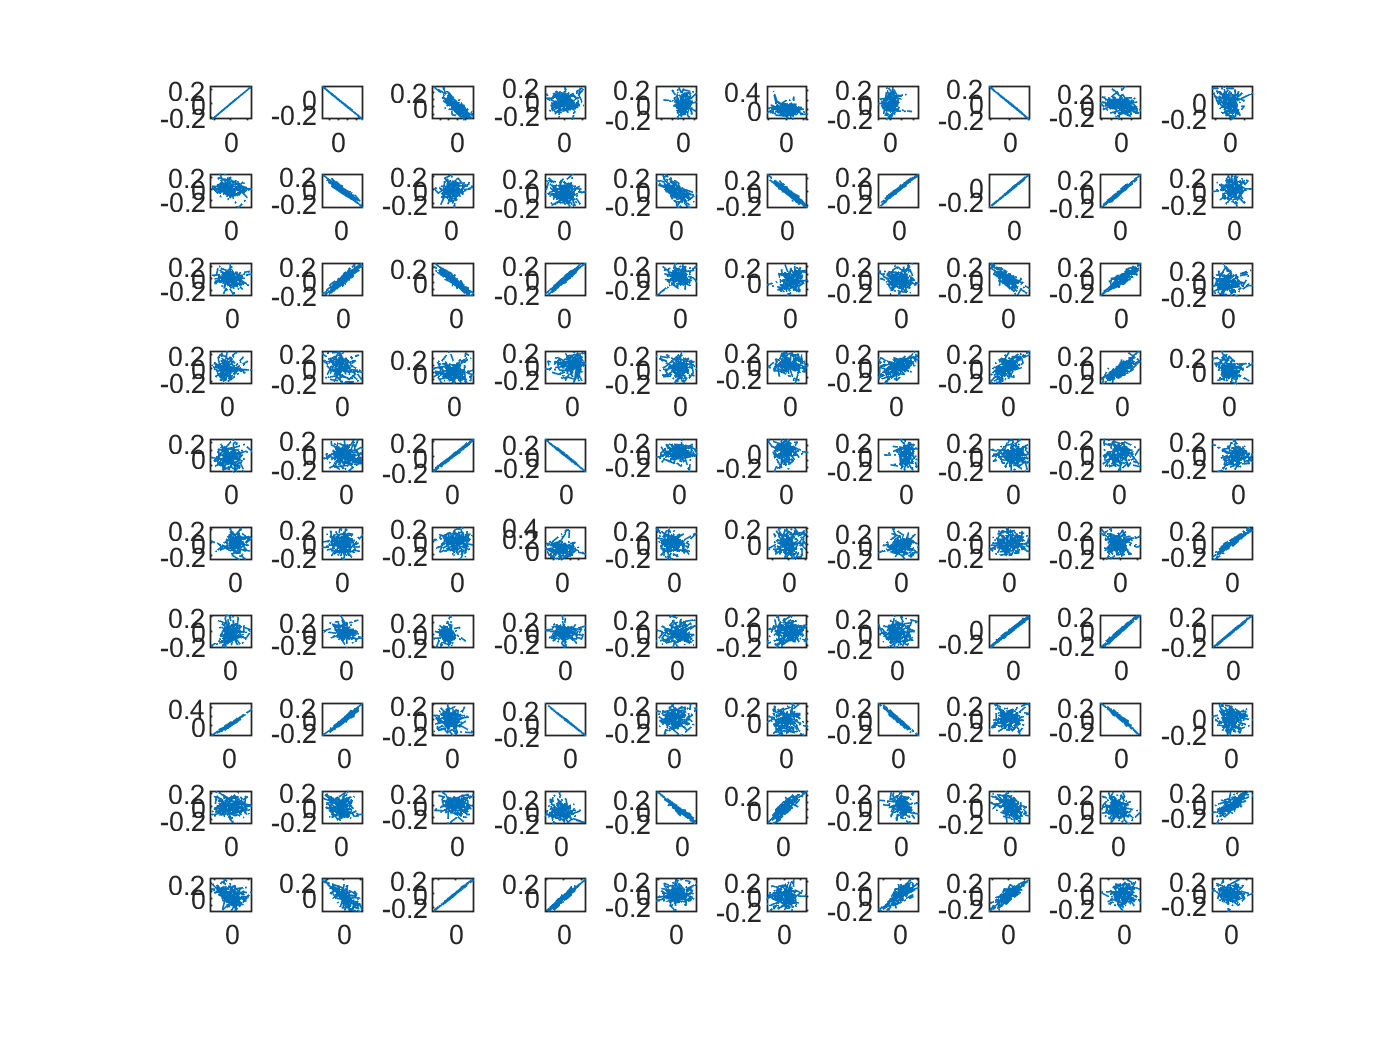
\includegraphics[width=\columnwidth]{figures/eigenvectorlowlowacc.png}           
                        \caption{Accuracy of Eigenvector Estimation Compared to MATLAB - Termination Condition=$10^{-3}$}                
                           \label{fig:eigenvectorlowlowacc}
         \end{figure}

   From Figure \ref{fig:eigenvaluelowlowacc} and Figure \ref{fig:eigenvectorlowlowacc}, the dramatic amount of loss of accuracy can be easily observed.
\subsection{Wigner's Semicircle Law}
\paragraph{} Wigner's Semicircle Law states that as $N \rightarrow \infty$, the probability that an eigenvalue $\lambda$ is
in the interval of $(\sqrt{N}x_1 < \lambda < \sqrt{N}x_2)$ is:
\begin{equation*}
   P(x_1 < \frac{\lambda}{\sqrt{N}} < x_2) = \frac{1}{2\pi}\int_{x_1}^{x_2} \sqrt{4-x^2}\,dx 
\end{equation*}
When the integration is done, the results can be displayed as following:
\begin{equation*}
   P(x_1 < \frac{\lambda}{\sqrt{N}} < x_2) = \frac{1}{2\pi} \left[ \frac{1}{2}\sqrt{4-{x_2}^2}x_2 + 2 \arcsin\frac{x_2}{2} - \frac{1}{2}\sqrt{4-{x_1}^2}x_1 + 2 \arcsin\frac{x_1}{2} \right]
\end{equation*}
\paragraph{} When we plot the probability distribution of the eigenvalues that is obtained by MATLAB, and the estimate of the Wigner's Semicircle Law for $N = 512, \;1024, \; 2048$, we obtain the following Figure \ref{fig:n512},Figure \ref{fig:n1024}, and Figure \ref{fig:n2048}.

\begin{figure}[H] 
   \centering 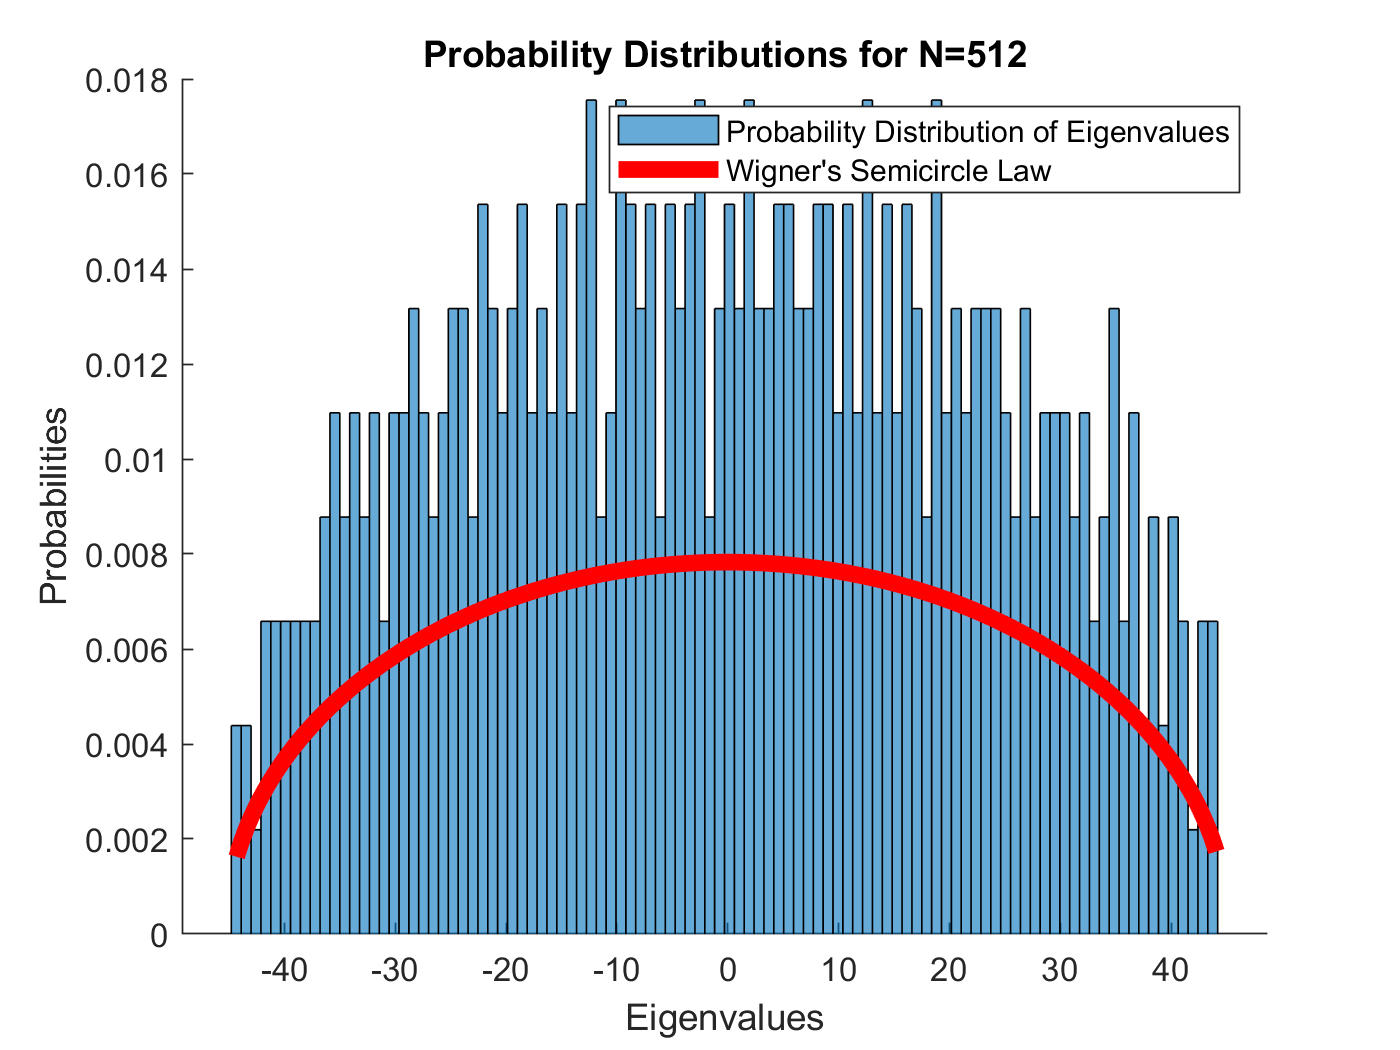
\includegraphics[width=0.7\columnwidth]{figures/n512.png}           
                  \caption{Probability distribution for $N=512$}                
                     \label{fig:n512}
   \end{figure}

\begin{figure}[H] 
   \centering 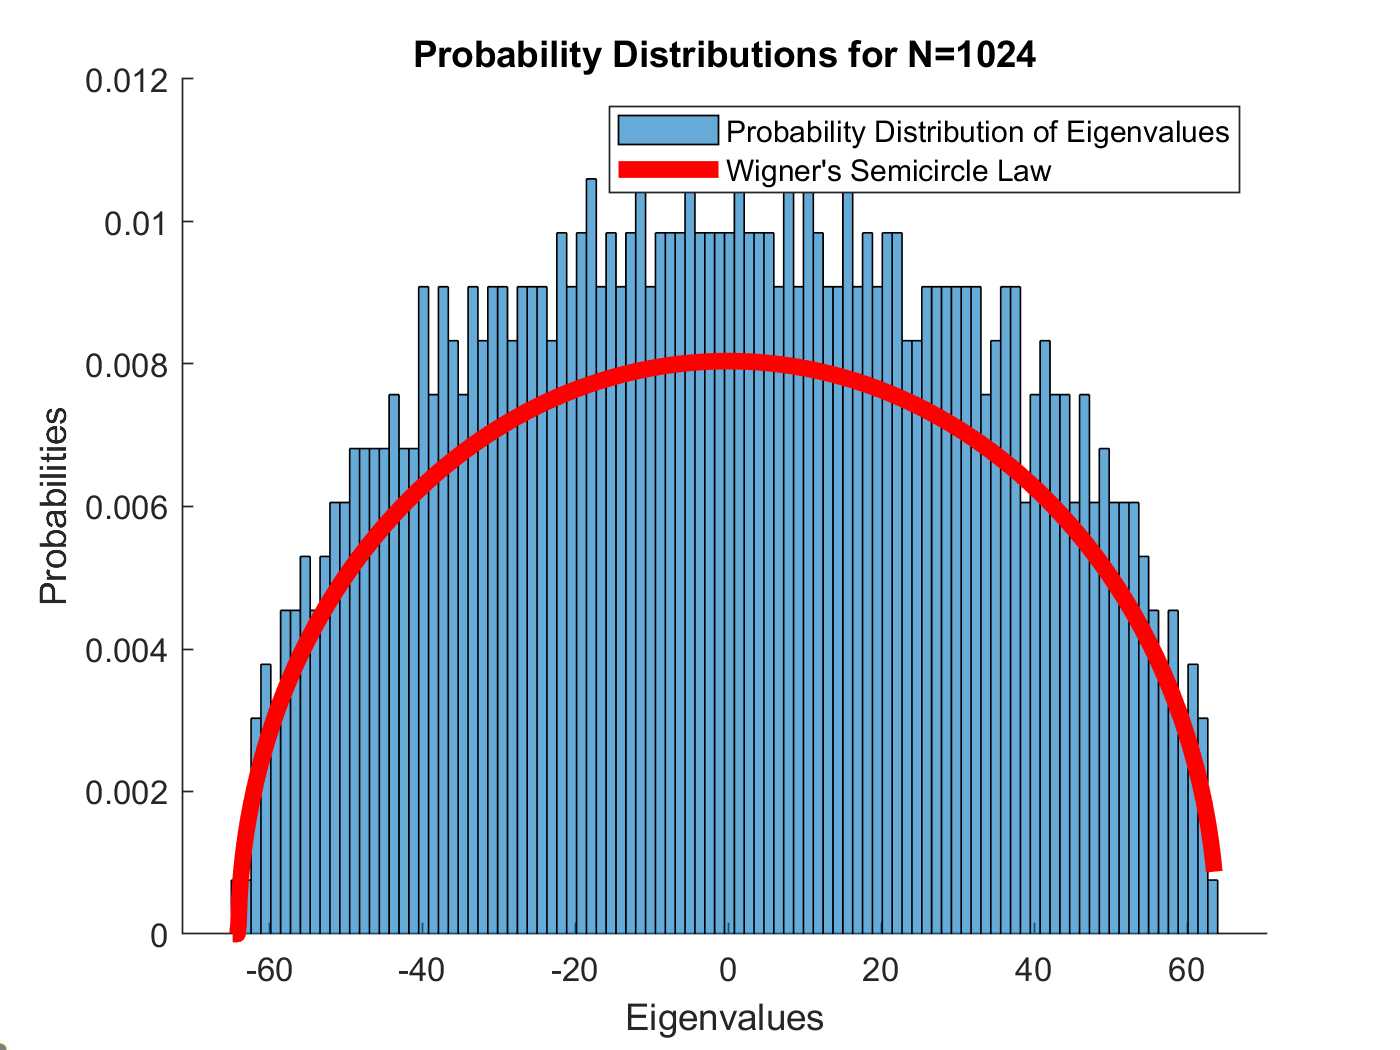
\includegraphics[width=0.7\columnwidth]{figures/n1024.png}           
                  \caption{Probability distribution for $N=1024$}                
                     \label{fig:n1024}
   \end{figure}

\begin{figure}[H] 
   \centering 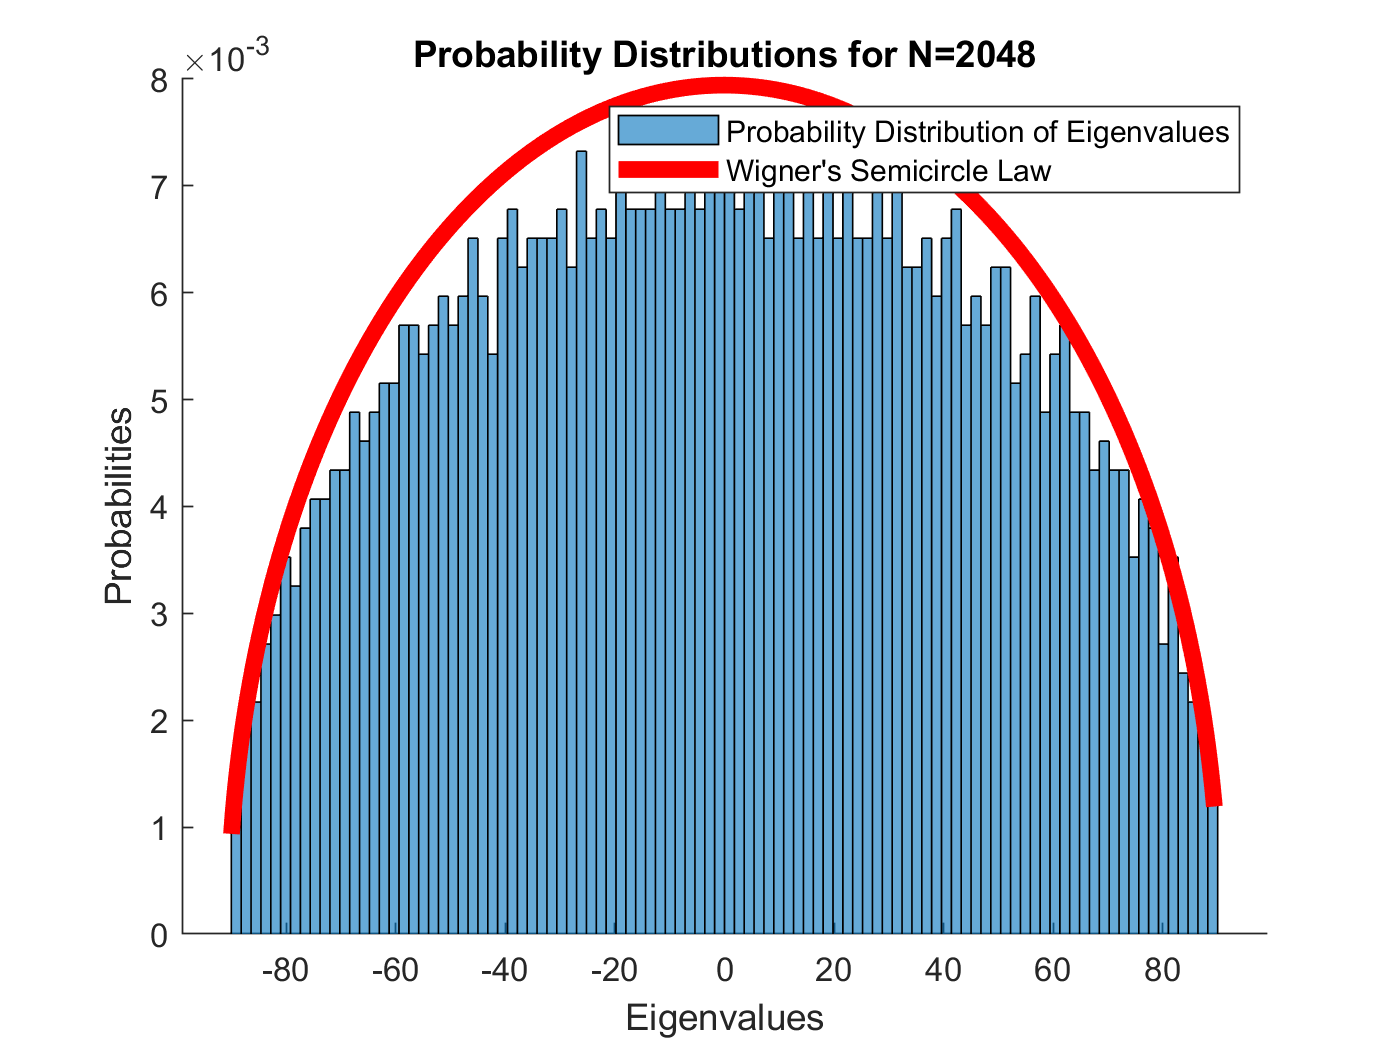
\includegraphics[width=0.7\columnwidth]{figures/n2048.png}           
                  \caption{Probability distribution for $N=2048$}                
                     \label{fig:n2048}
   \end{figure}
\end{document}

              


